\documentclass[11pt]{article}

\usepackage[margin=1in]{geometry}
\usepackage{amsmath,amssymb}
\usepackage{booktabs}
\usepackage{graphicx}
\usepackage{hyperref}

\title{Single-cell splicing analysis with proximal NND models}
\author{}
\date{}

\begin{document}
\maketitle

\section{Data objects}

The prompt-provided Zenodo object,
\texttt{splice\_adata\_for\_figures\_mouse\_foundation.h5ad}, is a fitted
mouse splicing atlas.  It contains cell metadata, learned cell program scores
\(\texttt{obsm["X\_PHI"]}\), and learned junction loadings
\(\texttt{varm["psi\_learned"]}\), but it does not contain the raw count layers
needed to construct per-cell PSI estimates.  In this object, the learned cell
program matrix has shape \(142315 \times 20\), and the learned junction loading
matrix has shape \(70102 \times 20\).  Equivalently, the cell metadata contains
columns \(\texttt{SP\_1},\ldots,\texttt{SP\_20}\).  Thus the fitted mouse atlas
has 20 splicing programs.

The raw count object used for model fitting was
\[
\texttt{/media/david/HDD/splicing\_data/model\_ready\_aligned\_splicing\_data\_20251009\_024406.h5ad}.
\]
This object has shape \(142315 \times 89831\).  Its \(\texttt{X}\) matrix,
\(\texttt{layers["cell\_by\_junction\_matrix"]}\), and
\(\texttt{layers["cell\_by\_cluster\_matrix"]}\) are all stored as HDF5-backed
CSR matrices.  Because the count layers contain about \(1.28\times 10^9\)
nonzero entries, the analysis avoids loading the full AnnData object with
\texttt{ad.read\_h5ad}.  Instead, selected row and column blocks are read
directly from the CSR arrays \(\texttt{data}\), \(\texttt{indices}\), and
\(\texttt{indptr}\) using \texttt{h5py}.

\section{Block selection}

The analysis first selects a manageable dense modeling block from the sparse
count object.  Cells are sampled from finite-coverage cells, weighted by
\(\texttt{total\_junction\_reads}\).  Junctions are selected among high-coverage
features using \(\texttt{n\_cells\_detected}\), retaining junctions whose
\(\texttt{event\_id}\) belongs to a multi-junction LeafCutter/ATSE cluster.
For each selected cell \(i\) and junction \(j\), the numerator count is
\[
k_{ij} = \texttt{cell\_by\_junction\_matrix}_{ij},
\]
and the denominator is
\[
n_{ij} = \texttt{cell\_by\_cluster\_matrix}_{ij}.
\]
The denominator is the total count for the corresponding local splicing
cluster, so \(k_{ij}/n_{ij}\) is the observed inclusion fraction for that
junction whenever \(n_{ij}>0\).

\section{Beta-binomial PSI estimates}

For each junction \(j\), a simple beta-binomial model is fit across cells:
\[
k_{ij}\mid n_{ij},p_{ij} \sim \operatorname{Binomial}(n_{ij},p_{ij}),
\qquad
p_{ij}\sim \operatorname{Beta}(\alpha_j,\beta_j).
\]
The parameters \((\alpha_j,\beta_j)\) are estimated by maximum likelihood,
parameterized by a mean and concentration.  Given the fitted prior, the
posterior parameters for an observed cell--junction pair are
\[
a_{ij}=k_{ij}+\alpha_j,\qquad
b_{ij}=n_{ij}-k_{ij}+\beta_j.
\]
The posterior PSI mean and standard error are
\[
\widehat{\psi}_{ij}
  = \frac{a_{ij}}{a_{ij}+b_{ij}},
\qquad
\widehat{\operatorname{se}}(\psi_{ij})
  =
  \left\{
  \frac{a_{ij}b_{ij}}
  {(a_{ij}+b_{ij})^2(a_{ij}+b_{ij}+1)}
  \right\}^{1/2}.
\]
The proximal Gaussian models are fit on the logit scale:
\[
Y_{ij}=\operatorname{logit}(\widehat{\psi}_{ij}).
\]
The standard error is transformed by the delta method,
\[
S_{ij}
  =
  \frac{\widehat{\operatorname{se}}(\psi_{ij})}
       {\widehat{\psi}_{ij}(1-\widehat{\psi}_{ij})}.
\]
Entries with \(n_{ij}=0\) are treated as missing.

\section{Proximal model comparison}

Observed entries are split into train, validation, and test sets.  The
regularization parameter is selected by validation RMSE on held-out observed
entries.  Final performance is reported on an independent test split, both on
the logit scale and after transforming predictions back to PSI.

Three proximal NND models are compared.

\subsection{Scaling the proximal algorithm}

The dense proximal implementation stores \(Y\), \(X\), FISTA auxiliary arrays,
and SVD work arrays as dense \(m\times n\) matrices.  For the full splicing
object, \(m=142315\) and \(n=89831\), so one float32 dense matrix is about
51 GB.  Repeated dense SVDs at this scale are not viable.

The scalable implementation instead represents the iterate \(X\) in low-rank
form,
\[
X = U\operatorname{diag}(d)V^\top,
\]
and stores the observations as a sparse CSR matrix.  For the homoskedastic
observed-entry loss with unit step size, the proximal-gradient update is
\[
X^{+}
=
\operatorname{SVT}_{\lambda}
\left\{
X - P_{\Omega}(X-Y)
\right\}
=
\operatorname{SVT}_{\lambda}
\left\{
X + P_{\Omega}(Y-X)
\right\}.
\]
The matrix inside the singular-value thresholding operator is therefore a
low-rank matrix plus a sparse correction.  The code exposes this object as a
\texttt{scipy.sparse.linalg.LinearOperator}; matrix-vector products are
\[
v \mapsto U\operatorname{diag}(d)(V^\top v) + C v,
\qquad
u \mapsto V\operatorname{diag}(d)(U^\top u) + C^\top u,
\]
where \(C=P_{\Omega}(Y-X)\) is sparse.  A truncated sparse SVD is then computed
with \texttt{svds}, and singular values below \(\lambda\) are thresholded away.
Thus neither \(X\) nor the filled-in matrix is ever materialized densely.

The ARPACK SVD backend was then replaced by a randomized SVD backend over the
same \texttt{LinearOperator}.  Given a Gaussian test matrix \(\Omega\), the
algorithm forms \(Q=\operatorname{qr}(A\Omega)\), applies one optional power
iteration with \(A^\top Q\) and \(A(A^\top Q)\), and computes the small SVD of
\(Q^\top A\).  On the full splicing matrix, this reduced a rank-20 proximal
iteration from roughly 2--3 minutes with ARPACK to about 37--40 seconds for the
homoskedastic runs after the first iteration.

The full sparse logit-PSI cache contains the CSR \(\texttt{indptr}\),
\(\texttt{indices}\), logit-PSI values, and logit-SE values as memory-mapped
arrays on the HDD.  The cache is about 15 GB and covers all
\(1{,}280{,}029{,}347\) observed entries.

\subsection{Scalable Taylor scoring}

Exact Taylor ELBO and LOO scoring would require row-wise covariance calculations
in \(n=89831\) dimensions, which is not tractable.  The full-matrix scorer
therefore uses a diagonal Taylor approximation from the low-rank fitted factors.
If \(X=U\operatorname{diag}(d)V^\top\), the prior curvature diagonal is
approximated by
\[
r_j
=
\lambda
\sum_{\ell}
\frac{V_{j\ell}^2}{\max(d_\ell,\epsilon)}.
\]
For an observed entry with observation variance \(v_{ij}\), the diagonal
posterior precision approximation is
\[
q_{ij}=v_{ij}^{-1}+r_j.
\]
The diagonal Taylor ELBO surrogate uses the observed Gaussian data term, the
diagonal log-determinant term \(\frac12\sum_{(i,j)\in\Omega}\log q_{ij}\), and
the nuclear norm penalty.  The LOO surrogate uses the local leverage
\[
h_{ij}=v_{ij}^{-1}/q_{ij}
\]
and reports the RMSE of \(e_{ij}/(1-h_{ij})\).  These scores are scalable and
use all observed entries, but they are diagonal approximations rather than the
exact row-covariance Taylor scores.

An intermediate approximation keeps row-wise covariance structure in the fitted
low-rank subspace and uses an isotropic completion off that subspace.  Write the
right singular vectors of the fitted matrix as \(V\) and the retained singular
values as \(d_\ell\).  The completed Gram approximation is
\[
X^\top X
\approx
V\operatorname{diag}(d_\ell^2)V^\top
+ \delta^2(I-VV^\top),
\]
with \(\delta=\max_\ell d_\ell\) by default.  The Taylor prior precision is then
\[
B
=
\lambda V\operatorname{diag}(d_\ell^{-1})V^\top
+ \lambda\delta^{-1}(I-VV^\top)
=
\tau I + VCV^\top,
\qquad
\tau=\lambda/\delta.
\]
For row \(i\), let \(D_i\) be the diagonal matrix of observed precisions in that
row.  The row covariance approximation is
\[
\Sigma_i = (D_i+B)^{-1}.
\]
This is evaluated by Woodbury in the retained rank \(r\), using the sparse
observed columns in each row.  The cost is proportional to the number of
observed entries in the scored rows times \(r^2\), so the current implementation
uses random row subsampling for scoring.  In the run below, 10000 rows were
sampled, covering about \(8.94\times 10^7\) observed entries.

\paragraph{Homoskedastic model.}
This model ignores the beta-binomial standard errors in the \(X\)-update and
estimates a single residual variance:
\[
Y_{ij}\mid X_{ij},\gamma^2 \sim N(X_{ij},\gamma^2),
\qquad
X\mid\gamma^2 \sim \operatorname{NND}(\lambda/\sqrt{\gamma^2}).
\]
The matrix \(X\) is updated by nuclear-norm proximal gradient, and
\(\gamma^2\) is updated using the Taylor/Hutchinson approximation described in
the homoskedastic noise derivation.

\paragraph{Heteroskedastic model.}
This model uses the beta-binomial delta-method standard errors as known
observation noise:
\[
Y_{ij}\mid X_{ij},S_{ij} \sim N(X_{ij},S_{ij}^2).
\]
It solves
\[
\min_X
\frac12\sum_{(i,j)\in\Omega}
\frac{(Y_{ij}-X_{ij})^2}{S_{ij}^2}
+\lambda\|X\|_*.
\]

\paragraph{Combined model.}
This model uses the beta-binomial standard errors but also estimates an
additional homoskedastic residual variance \(g\):
\[
Y_{ij}\mid X_{ij},S_{ij},g
\sim N(X_{ij},S_{ij}^2+g).
\]
The \(X\)-update is the same efficient proximal update with effective standard
errors \((S_{ij}^2+g)^{1/2}\).  The scalar \(g\) is updated by a Taylor
diagonal-variance approximation, using Hutchinson probes for the trace terms
when requested.  The analysis grids over the effective nuclear-norm penalty
rather than jointly estimating \(\lambda\) and \(g\).

\section{Debug runs}

The main real-data debug run used a \(600\times 200\) block, 40 proximal
iterations, and the lambda grid
\[
\{0.01,0.03,0.1,0.3,1\}.
\]
Sparse block extraction took about 11 seconds, beta-binomial PSI fitting about
1 second, and the proximal model comparison about 94 seconds.

\begin{center}
\begin{tabular}{lrrrr}
\toprule
model & selected \(\lambda\) & test logit RMSE & test PSI RMSE & noise estimate\\
\midrule
homoskedastic & 1.00 & 1.665 & 0.118 & \(\gamma^2=0.00441\)\\
heteroskedastic & 0.03 & 5.020 & 0.381 & --\\
combined & 1.00 & 4.692 & 0.297 & \(g=0.00407\)\\
\bottomrule
\end{tabular}
\end{center}

On this block, the homoskedastic model performed best.  The heteroskedastic and
combined models were much worse, suggesting that the delta-method standard
errors from the simple per-junction beta-binomial fit are not yet calibrated
well enough on the logit scale, or that some high-precision entries are being
overweighted relative to the low-rank signal.

\subsection{All-cell, top-junction run}

The literal full \(142315\times 89831\) proximal problem is not run as a dense
matrix problem: it would require materializing many \(12.8\) billion-entry
arrays and repeatedly computing SVDs.  Instead, the full-cell run uses all
142315 cells and the top 20 high-coverage selected junctions.  This keeps the
cell axis complete while limiting the dense proximal block to
\(142315\times 20\).  The same lambda grid
\(\{0.01,0.03,0.1,0.3,1\}\) and 40 proximal iterations were used.  Sparse block
extraction took about 109 seconds, beta-binomial PSI fitting about 10 seconds,
proximal model comparison about 81 seconds, and the all-cell splicing-program
cell-type classifiers about 152 seconds.

\begin{center}
\begin{tabular}{lrrrr}
\toprule
model & selected \(\lambda\) & test logit RMSE & test PSI RMSE & noise estimate\\
\midrule
homoskedastic & 1.00 & 2.319 & 0.083 & \(\gamma^2=5.40\times10^{-5}\)\\
heteroskedastic & 0.03 & 5.174 & 0.420 & --\\
combined & 1.00 & 3.846 & 0.173 & \(g=0.450\)\\
\bottomrule
\end{tabular}
\end{center}

The all-cell top-junction result again favors the homoskedastic model.  The
combined model improves substantially over the heteroskedastic-only model but
still does not match the homoskedastic fit on held-out PSI RMSE.

\subsection{Literal full observed-matrix sparse proximal run}

The sparse-plus-low-rank implementation was run on the literal full observed
matrix, with shape \(142315\times 89831\) and \(1{,}280{,}029{,}347\) observed
entries.  The first cache construction streamed the whole HDF5 count object to
fit per-junction beta moments and write logit-PSI/logit-SE memmaps.  Subsequent
proximal runs reuse this cache.

With rank cap 20 and \(\lambda=10000\), the first three full sparse SVT
iterations took 127, 130, and 157 seconds, respectively.  Continuing for three
more iterations from the saved factors took 154, 127, and 152 seconds.  The
retained rank shrank from 6 after the first update to 2 after six updates, and
the final observed logit RMSE was 2.145.

With rank cap 30 and \(\lambda=5000\), the first two full sparse SVT iterations
took 226 and 192 seconds.  The retained rank was 19 after the first update and
14 after the second update, with final observed logit RMSE 2.575.  This lower
penalty preserves more splicing structure but needs additional iterations for a
fair comparison with the longer \(\lambda=10000\) run.

With the randomized SVD backend, a one-step lambda sweep over
\(\lambda\in\{5000,10000\}\) was run for the homoskedastic, heteroskedastic, and
combined noise models.  Within each noise model, the diagonal Taylor ELBO
selected \(\lambda=5000\).  The diagonal LOO surrogate also selected
\(\lambda=5000\) for the homoskedastic and combined models; for the
heteroskedastic model the LOO scores for 5000 and 10000 were very close, with a
slight preference for 10000 after one step.

Using the ELBO-selected \(\lambda=5000\), three randomized proximal iterations
were run for each noise model.  The corrected homoskedastic score estimates
\(\gamma^2\) from the final residuals for scoring, while treating \(\lambda\) as
the effective proximal penalty during fitting.

\begin{center}
\begin{tabular}{lrrrrr}
\toprule
model & rank & obs. logit RMSE & diag. LOO RMSE & diag. Taylor ELBO & noise\\
\midrule
homoskedastic & 10 & 2.335 & 231.3 & \(-1.856\times 10^9\) & \(\gamma^2=5.45\)\\
heteroskedastic & 18 & 4.596 & 320.5 & \(-1.727\times 10^9\) & --\\
combined & 18 & 4.548 & 368.6 & \(-1.624\times 10^9\) & \(g\approx 10^{-6}\)\\
\bottomrule
\end{tabular}
\end{center}

The diagonal Taylor ELBO favors the combined model, while the diagonal LOO
surrogate and direct observed-entry reconstruction favor the homoskedastic
model.  Because the ELBO and LOO scores here use a diagonal approximation to the
Taylor covariance, this disagreement should be interpreted as a diagnostic:
the scalable scoring machinery is now in place, but the calibration of the
heteroskedastic standard errors and diagonal curvature approximation still needs
stress-testing.

The low-rank-plus-isotropic row covariance scorer was then evaluated on the same
\(\lambda=5000\) fits using 10000 sampled rows.

\begin{center}
\begin{tabular}{lrrrr}
\toprule
model & obs. logit RMSE & row-iso LOO RMSE & row-iso ELBO & seconds\\
\midrule
homoskedastic & 2.335 & 15.293 & \(1.767\times 10^{10}\) & 10.6\\
heteroskedastic & 4.595 & 5.958 & \(-1.992\times 10^9\) & 60.6\\
combined & 4.547 & 7.216 & \(1.066\times 10^9\) & 98.1\\
\bottomrule
\end{tabular}
\end{center}

This row-covariance LOO approximation is much less pathological than the purely
diagonal LOO approximation.  It favors the heteroskedastic model, despite its
worse raw reconstruction RMSE, because it accounts for posterior uncertainty in
the fitted low-rank subspace.  The row-iso ELBO contains a large isotropic
log-determinant contribution that differs strongly across noise models, so it
should not yet be used as the sole selection rule without additional calibration
or shared constants across model families.

\subsection{All-cell, selected 10000-junction run}

A larger all-cell subset was built by selecting 10000 junctions using both
coverage and variability across medium-resolution cell types.  For each
junction, counts were aggregated by \(\texttt{medium\_cell\_type}\), and the
cell-type PSI variability was computed from the cell-type-specific
\(\sum k/\sum n\) estimates.  Eligible junctions were required to belong to a
multi-junction event and to have sufficient denominator counts in at least 8
cell types.  Junctions were ranked by the sum of their percentile ranks for
\(\log(1+n_{\mathrm{cells\,detected}})\) and between-cell-type PSI variance.

The selected set contains 10000 junctions, spans 6497 splicing events and 4380
genes, and has median detection in 12338 cells.  The resulting all-cell sparse
cache has shape \(142315\times 10000\) with \(263{,}931{,}532\) observed
entries.

\begin{figure}[t]
\centering
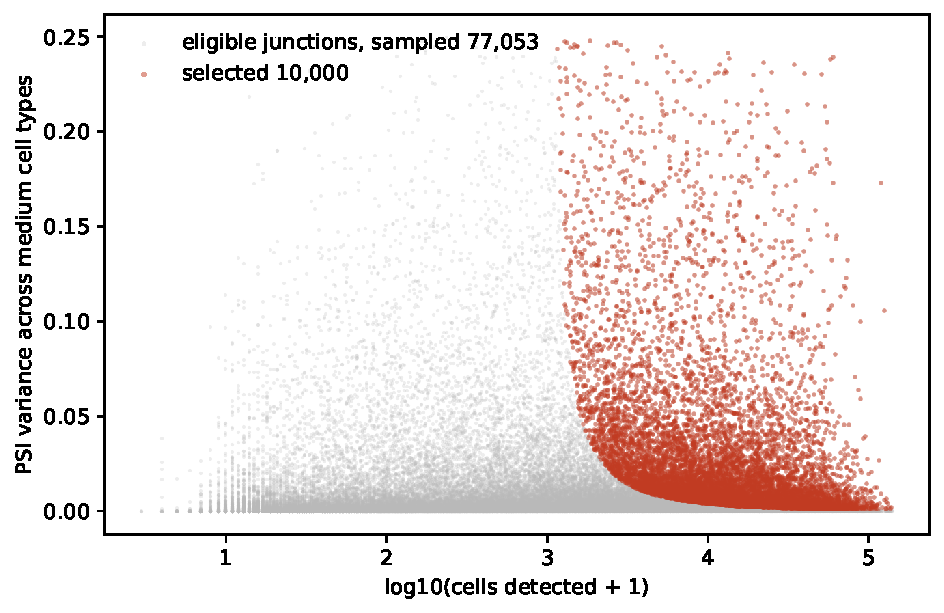
\includegraphics[width=0.75\linewidth]{figures/splicing_subset_junction_selection.pdf}
\caption{Selection of the 10000-junction subset.  Grey points are eligible
multi-junction features with sufficient medium-cell-type coverage; red points
are the selected junctions.  The selected subset emphasizes both coverage and
between-cell-type PSI variability.}
\label{fig:splicing-subset-selection}
\end{figure}

A one-step lambda sweep over \(\lambda\in\{1000,3000,5000,10000\}\) was run for
each noise model.  The longer follow-up fits used \(\lambda=1000\) for the
homoskedastic model, \(\lambda=3000\) for the heteroskedastic model, and
\(\lambda=1000\) for the combined model.  Each fit used 5 randomized proximal
iterations with rank cap 50.

\begin{center}
\begin{tabular}{lrrrrr}
\toprule
model & \(\lambda\) & rank & obs. logit RMSE & row-iso LOO RMSE & row-iso ELBO\\
\midrule
homoskedastic & 1000 & 13 & 1.534 & 26.749 & \(1.901\times 10^9\)\\
heteroskedastic & 3000 & 13 & 2.546 & 5.467 & \(-3.104\times 10^8\)\\
combined & 1000 & 2 & 2.115 & 9.779 & \(1.500\times 10^9\)\\
\bottomrule
\end{tabular}
\end{center}

The same pattern appears more cleanly on this subset: raw observed-entry RMSE
favors the homoskedastic model, while the low-rank-plus-isotropic row LOO score
favors the heteroskedastic model.  The combined model is intermediate by LOO and
raw RMSE.  Thus, when the selected junctions are chosen to be both covered and
cell-type-variable, the heteroskedastic uncertainty model looks more plausible
under the row-covariance predictive criterion even though it does not minimize
point-reconstruction error.

\begin{figure}[t]
\centering
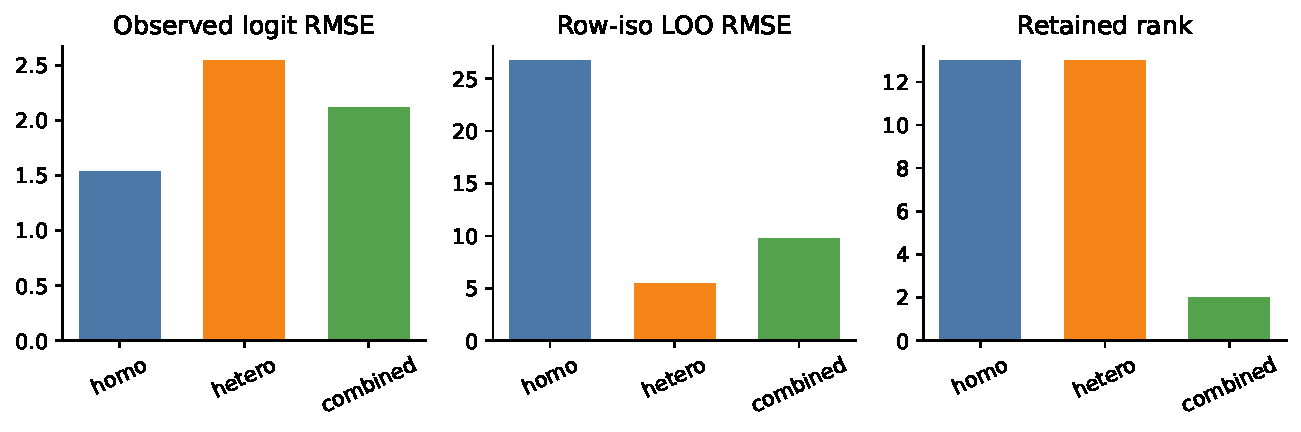
\includegraphics[width=0.9\linewidth]{figures/splicing_subset_model_scores.pdf}
\caption{Model comparison on all cells and the selected 10000-junction subset.
The homoskedastic model gives the best point reconstruction, while the
heteroskedastic model gives the best low-rank-plus-isotropic row LOO score.}
\label{fig:splicing-subset-model-scores}
\end{figure}

\subsection{Logit-space versus PSI-space fitting}

The sparse proximal runner was extended so that the same observed CSR pattern
can be fit either on
\[
Y_{ij}=\operatorname{logit}(\widehat\psi_{ij})
\]
or directly on the bounded PSI scale \(Y_{ij}=\widehat\psi_{ij}\).  The
PSI-space standard errors were obtained from the existing logit-scale standard
errors by the inverse delta-method relation
\[
S^{(\psi)}_{ij}
  =
  S^{(\operatorname{logit})}_{ij}
  \widehat\psi_{ij}(1-\widehat\psi_{ij}).
\]
For the PSI-space heteroskedastic model the regularization scale must be much
larger, because the smallest allowed variance was \(0.01^2\), giving a
proximal step size of \(10^{-4}\).  Thus a threshold of order 100 requires
\(\lambda\) of order \(10^6\).

The PSI-space all-cell, 10000-junction fits used \(\lambda=300\) for the
homoskedastic and combined models and \(\lambda=10^6\) for the heteroskedastic
model.  Each fit used 5 randomized proximal iterations with rank cap 50.  The
homoskedastic PSI fit retained rank 7, the heteroskedastic fit retained rank
13, and the combined fit reached the rank cap after \(g\) shrank and the
effective threshold dropped.

\begin{center}
\begin{tabular}{llrrrr}
\toprule
space & model & \(\lambda\) & rank & obs. RMSE & row-iso LOO RMSE\\
\midrule
logit & homoskedastic & 1000 & 13 & 1.534 & 26.749\\
logit & heteroskedastic & 3000 & 13 & 2.546 & 5.467\\
logit & combined & 1000 & 2 & 2.115 & 9.779\\
PSI & homoskedastic & 300 & 7 & 0.276 & 27.599\\
PSI & heteroskedastic & \(10^6\) & 13 & 0.539 & 3.198\\
PSI & combined & 300 & 50 & 0.259 & 25.928\\
\bottomrule
\end{tabular}
\end{center}

Observed-entry RMSE is not directly comparable across logit and PSI scales: the
PSI residual is bounded while the logit residual is not.  Within each fitted
space, however, the qualitative pattern is stable.  Homoskedastic or combined
fits give better point reconstruction, while the heteroskedastic model gives
the best low-rank-plus-isotropic row LOO score.  The combined PSI fit should be
interpreted cautiously because its retained rank is capped at 50, indicating
that joint \(g\) and low-rank fitting is again reducing the effective
regularization too aggressively.

The heteroskedastic PSI fit also exposed a practical step-size issue.  With a
hard SE floor of 0.01, the maximum precision is \(10^4\), so the global
proximal-gradient step is only \(10^{-4}\).  This is mathematically consistent
with the weighted Gaussian objective, but it makes the update nearly frozen by
a small number of very high-precision observations.  In the selected
10000-junction cache, the empirical PSI-SE quantiles are approximately 0.003
at 1\%, 0.052 at 25\%, and 0.101 at 50\%.  A follow-up run capped precision by
raising the floor to the first-quartile PSI-SE, 0.052.  With
\(\lambda=100000\), this increased the step to 0.00272, retained rank 7 after
five iterations, and gave observed PSI RMSE 0.375 with row-iso LOO RMSE 5.690.
A median floor moved faster and gave lower point RMSE, but it caps half of the
observed entries and is therefore a more aggressive change to the noise model.
Thus the tiny heteroskedastic step is not an SVD or warm-start issue; it is a
precision-capping issue.  Quantile SE floors should be treated as part of the
reported noise model.

\begin{figure}[t]
\centering
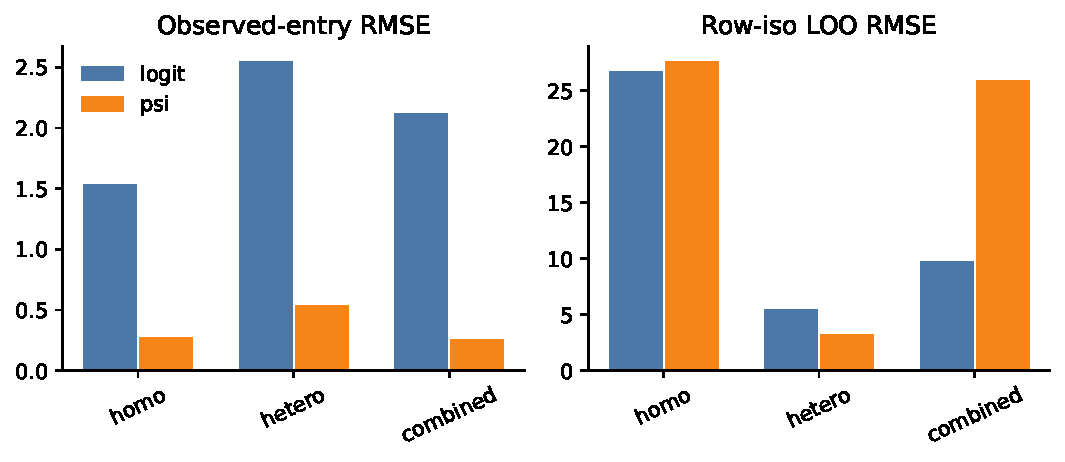
\includegraphics[width=0.82\linewidth]{figures/splicing_logit_vs_psi_model_scores.pdf}
\caption{Comparison of logit-space and PSI-space proximal fits on all cells
and the selected 10000-junction subset.  RMSE values are only comparable within
a value space; the row-iso LOO ordering favors the heteroskedastic uncertainty
model in both spaces.}
\label{fig:splicing-logit-vs-psi-scores}
\end{figure}

To visualize whether the fitted low-rank splicing spaces preserve cell-type
structure, UMAPs were computed from the atlas splicing programs and from fitted
cell factor scores \(U\operatorname{diag}(d)\).  The same 20000 sampled cells
were embedded in each panel and colored by broad cell type.  The UMAP and
junction-selection plots are rendered as PDFs with rasterized point layers and
subsampling, rather than pure vector graphics containing every point, to keep
the document size manageable.

\begin{figure}[t]
\centering
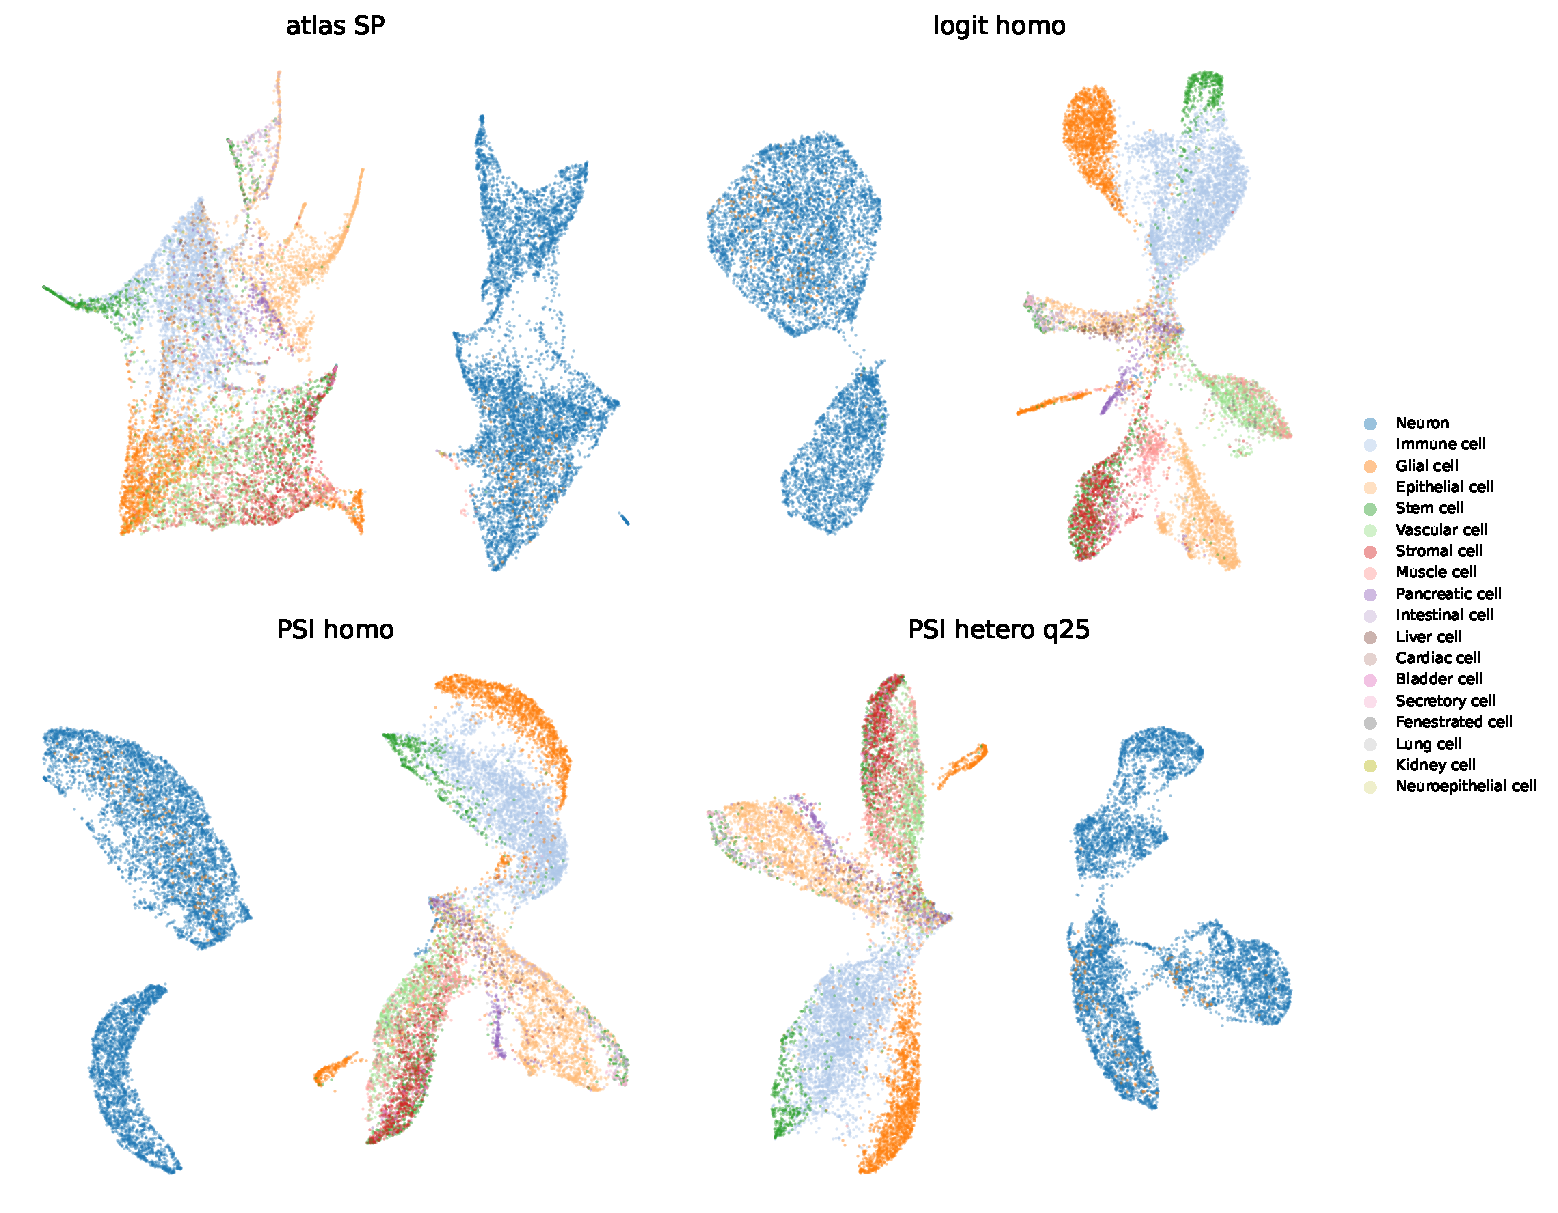
\includegraphics[width=\linewidth]{figures/splicing_space_umap_broad_cell_type.pdf}
\caption{UMAPs of splicing latent spaces colored by broad cell type.  The
panels compare the published atlas splicing programs, logit-space
homoskedastic factors, PSI-space homoskedastic factors, and PSI-space
heteroskedastic factors with a first-quartile SE floor.  All panels use the same
sampled cells.}
\label{fig:splicing-space-umap-logit-vs-psi}
\end{figure}

Cell-type separation was quantified directly in latent space using local
\(k\)-nearest-neighbor purity and silhouette.  For each embedding, 30000 cells
were sampled and each cell's 15 nearest neighbors were queried in the
standardized latent coordinates.  The reported enrichment divides the observed
same-label neighbor fraction by the same-label fraction expected from the label
frequencies alone.  Silhouette was computed on a 12000-cell subsample.

\begin{center}
\begin{tabular}{llrrr}
\toprule
embedding & label & local purity & enrichment & silhouette\\
\midrule
atlas SP & broad & 0.728 & 3.57 & -0.074\\
logit homo & broad & 0.851 & 4.17 & 0.019\\
PSI homo & broad & 0.818 & 4.01 & 0.021\\
PSI hetero q25 & broad & 0.815 & 4.00 & 0.006\\
atlas SP & medium & 0.563 & 6.62 & -0.097\\
logit homo & medium & 0.696 & 8.18 & -0.022\\
PSI homo & medium & 0.636 & 7.48 & -0.059\\
PSI hetero q25 & medium & 0.627 & 7.37 & -0.092\\
\bottomrule
\end{tabular}
\end{center}

The fitted proximal factors therefore show strong local cell-type structure:
broad-cell-type neighbor purity is about 0.81--0.85 for the fitted spaces
against a random-label baseline of 0.20, and medium-cell-type purity is about
0.62--0.70 against a baseline of 0.085.  Silhouette is small and becomes
negative for medium and specific labels, so the separation should be understood
as local manifold organization rather than clean globally separated clusters.

\begin{figure}[t]
\centering
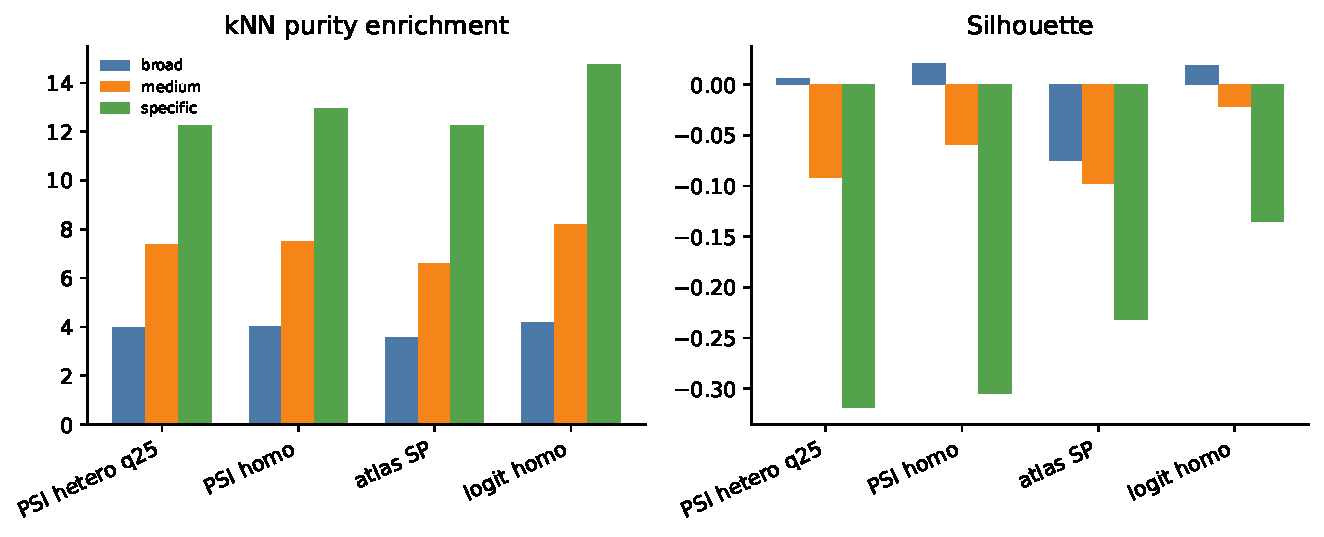
\includegraphics[width=0.82\linewidth]{figures/latent_celltype_separation_metrics.pdf}
\caption{Cell-type separation metrics in splicing latent spaces.  Local
neighbor purity shows strong enrichment for broad, medium, and specific labels;
silhouette is much weaker, indicating overlapping manifolds rather than
well-separated convex clusters.}
\label{fig:splicing-latent-celltype-separation}
\end{figure}

To interpret which factors drive broad cell-type organization, factor usage was
averaged within each broad cell type.  Cell-level factor scores were first
standardized within each embedding.  Because singular vectors are sign
ambiguous, each fitted factor was oriented so that the cell type with the
largest absolute mean usage is positive before plotting.

\begin{figure}[t]
\centering
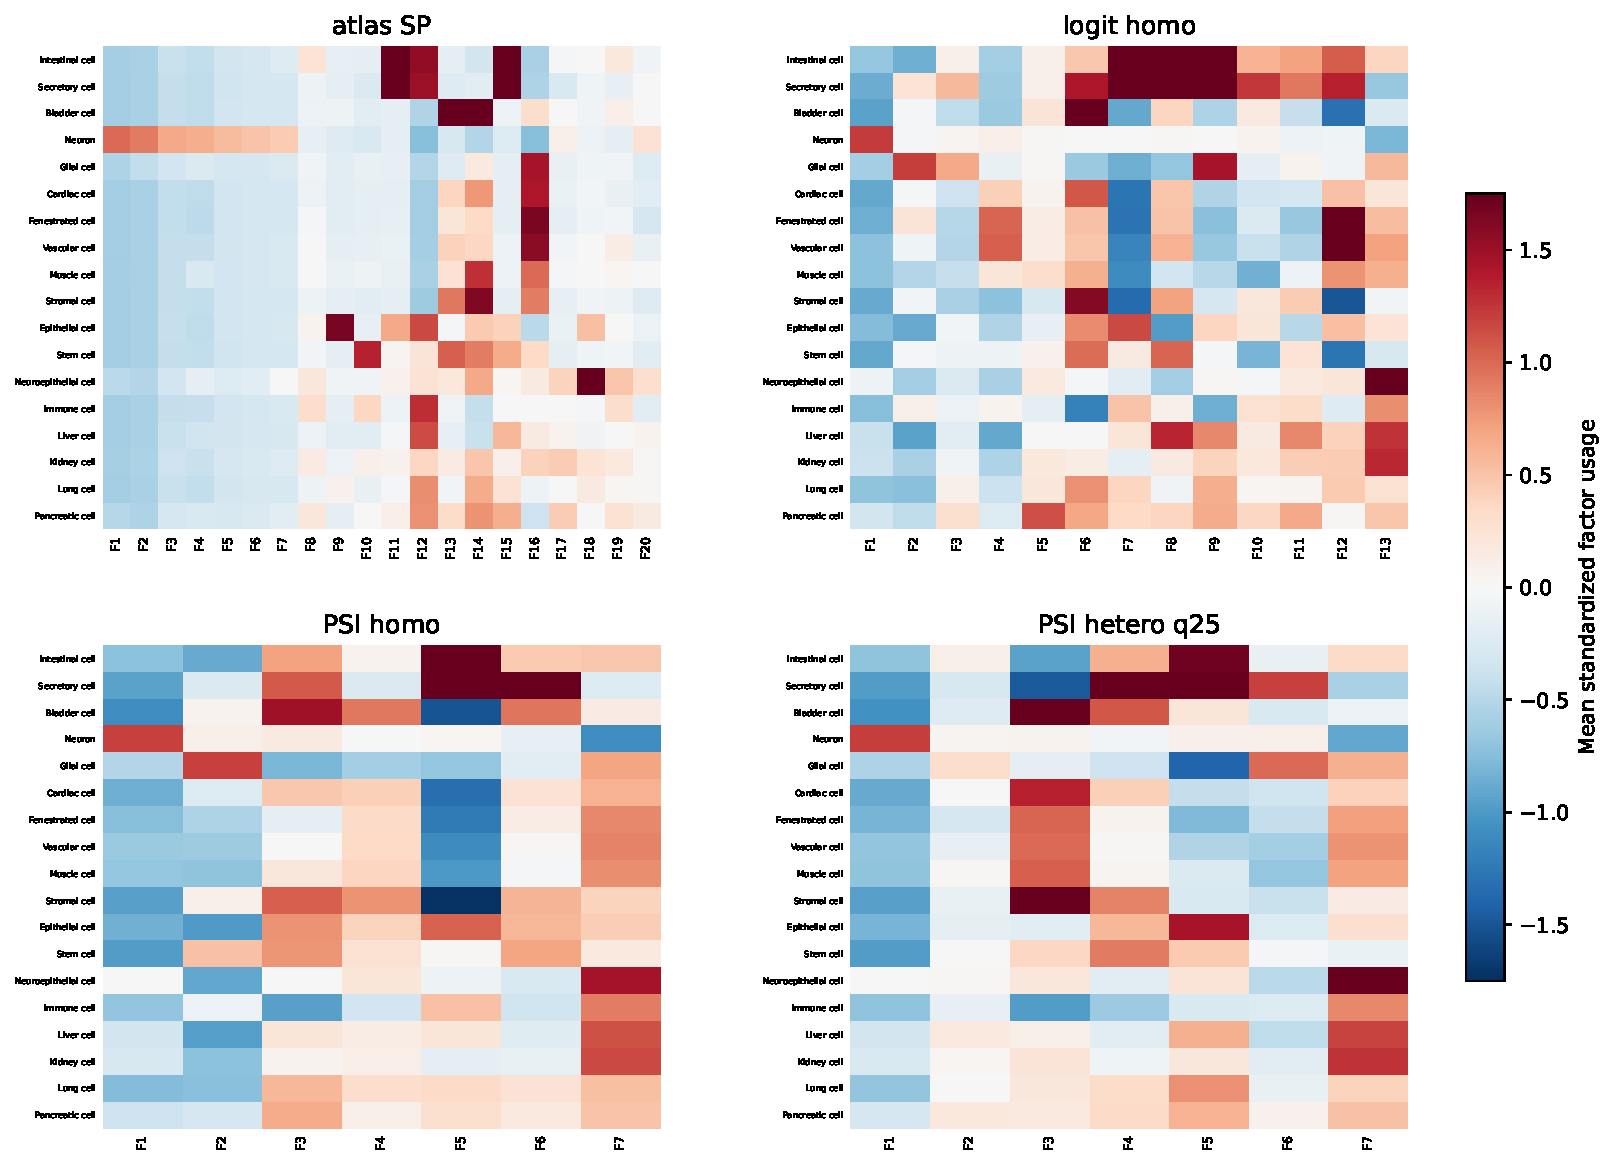
\includegraphics[width=\linewidth]{figures/broad_cell_type_factor_usage_heatmap.pdf}
\caption{Mean standardized factor usage by broad cell type.  Rows are broad
cell types ordered by clustering the atlas splicing-program means.  The panels
compare atlas splicing programs, logit-space homoskedastic factors, PSI-space
homoskedastic factors, and PSI-space heteroskedastic factors with a
first-quartile SE floor.}
\label{fig:splicing-celltype-factor-usage}
\end{figure}

\begin{figure}[p]
\centering
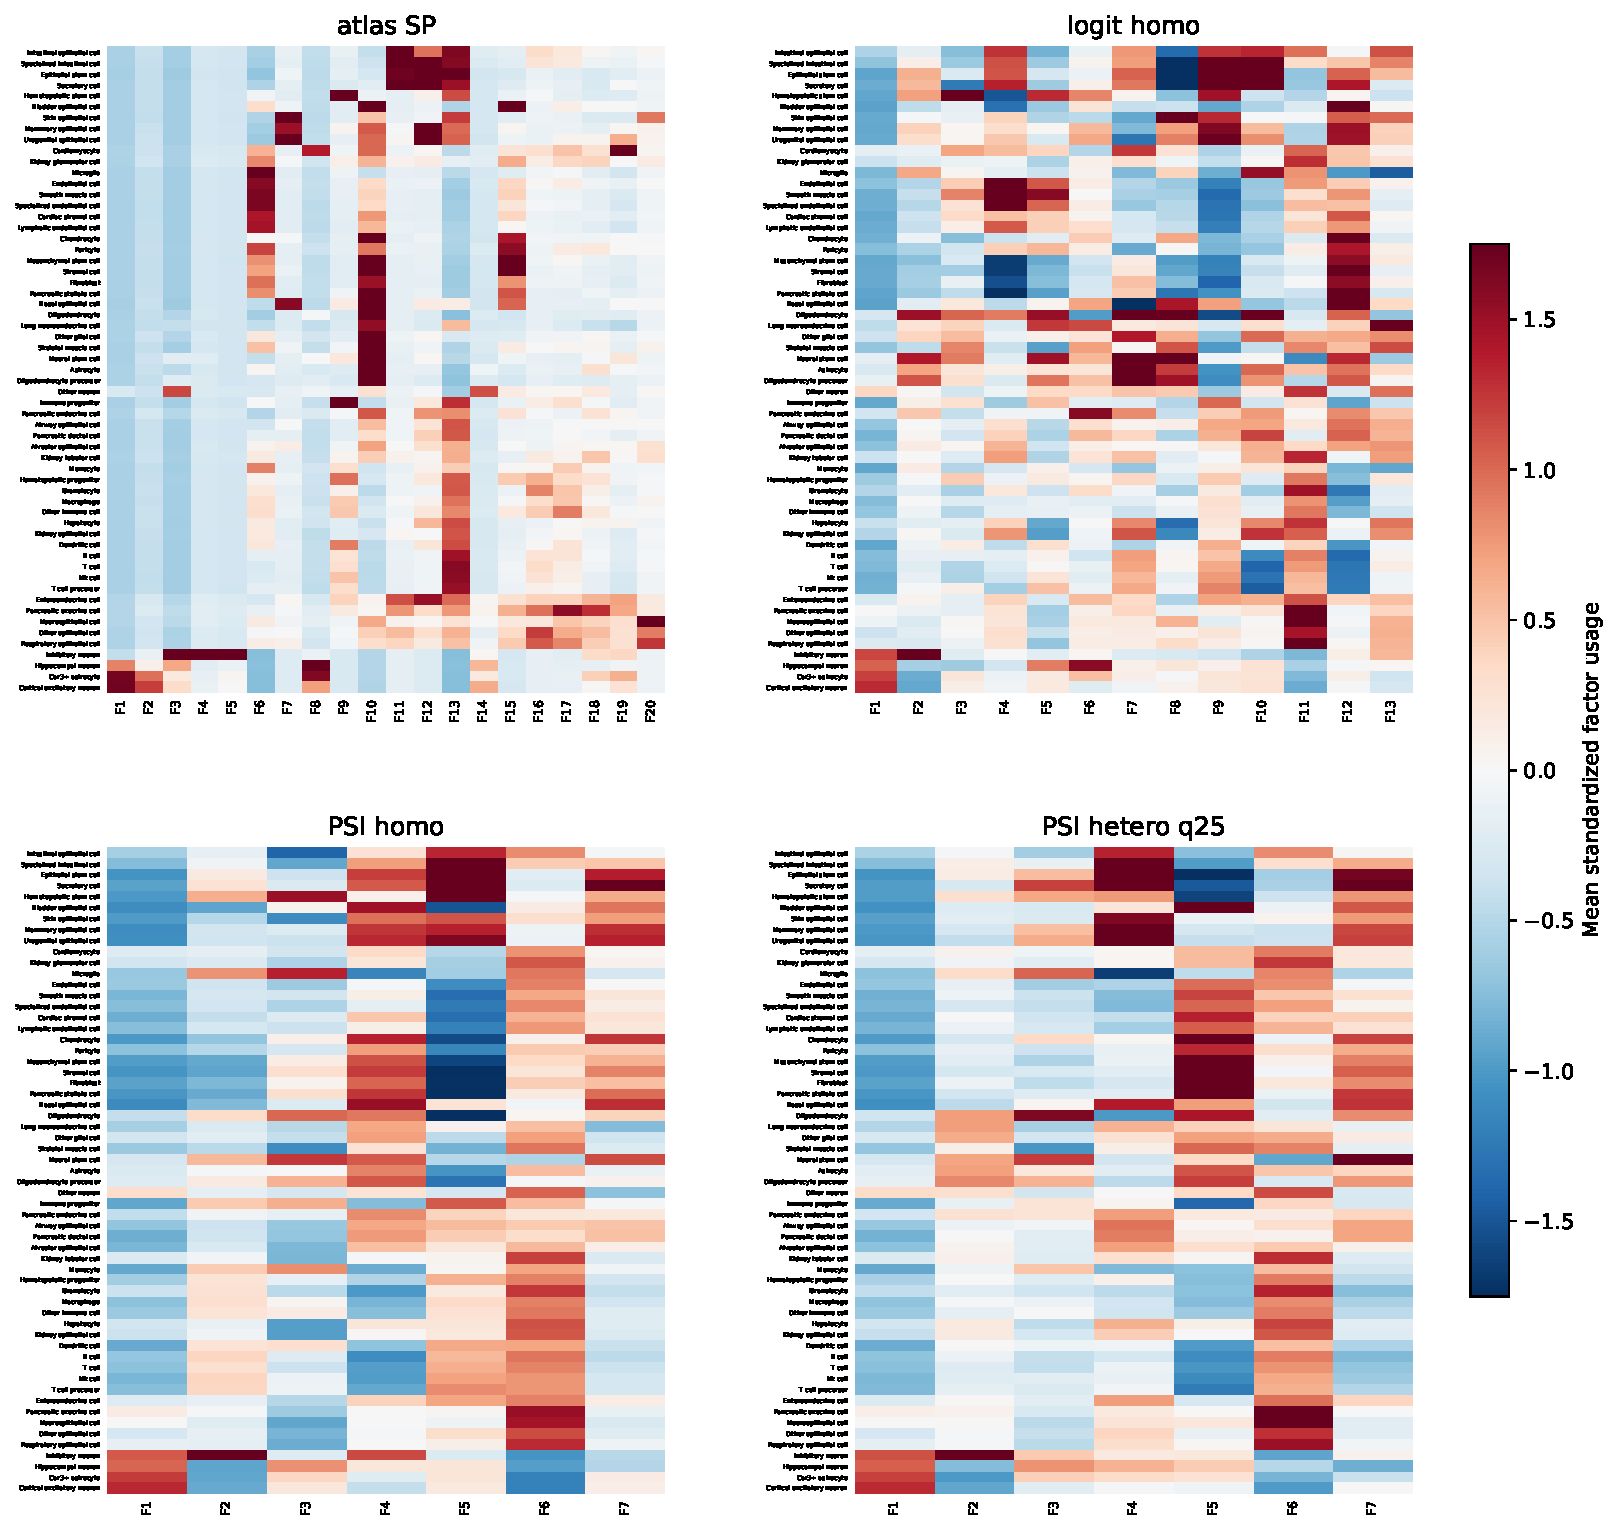
\includegraphics[width=\linewidth,height=0.9\textheight,keepaspectratio]{figures/medium_cell_type_factor_usage_heatmap.pdf}
\caption{Mean standardized factor usage by medium cell type.  The same factor
orientation and row-clustering convention as
Figure~\ref{fig:splicing-celltype-factor-usage} is used.}
\label{fig:splicing-medium-celltype-factor-usage}
\end{figure}

\begin{figure}[p]
\centering
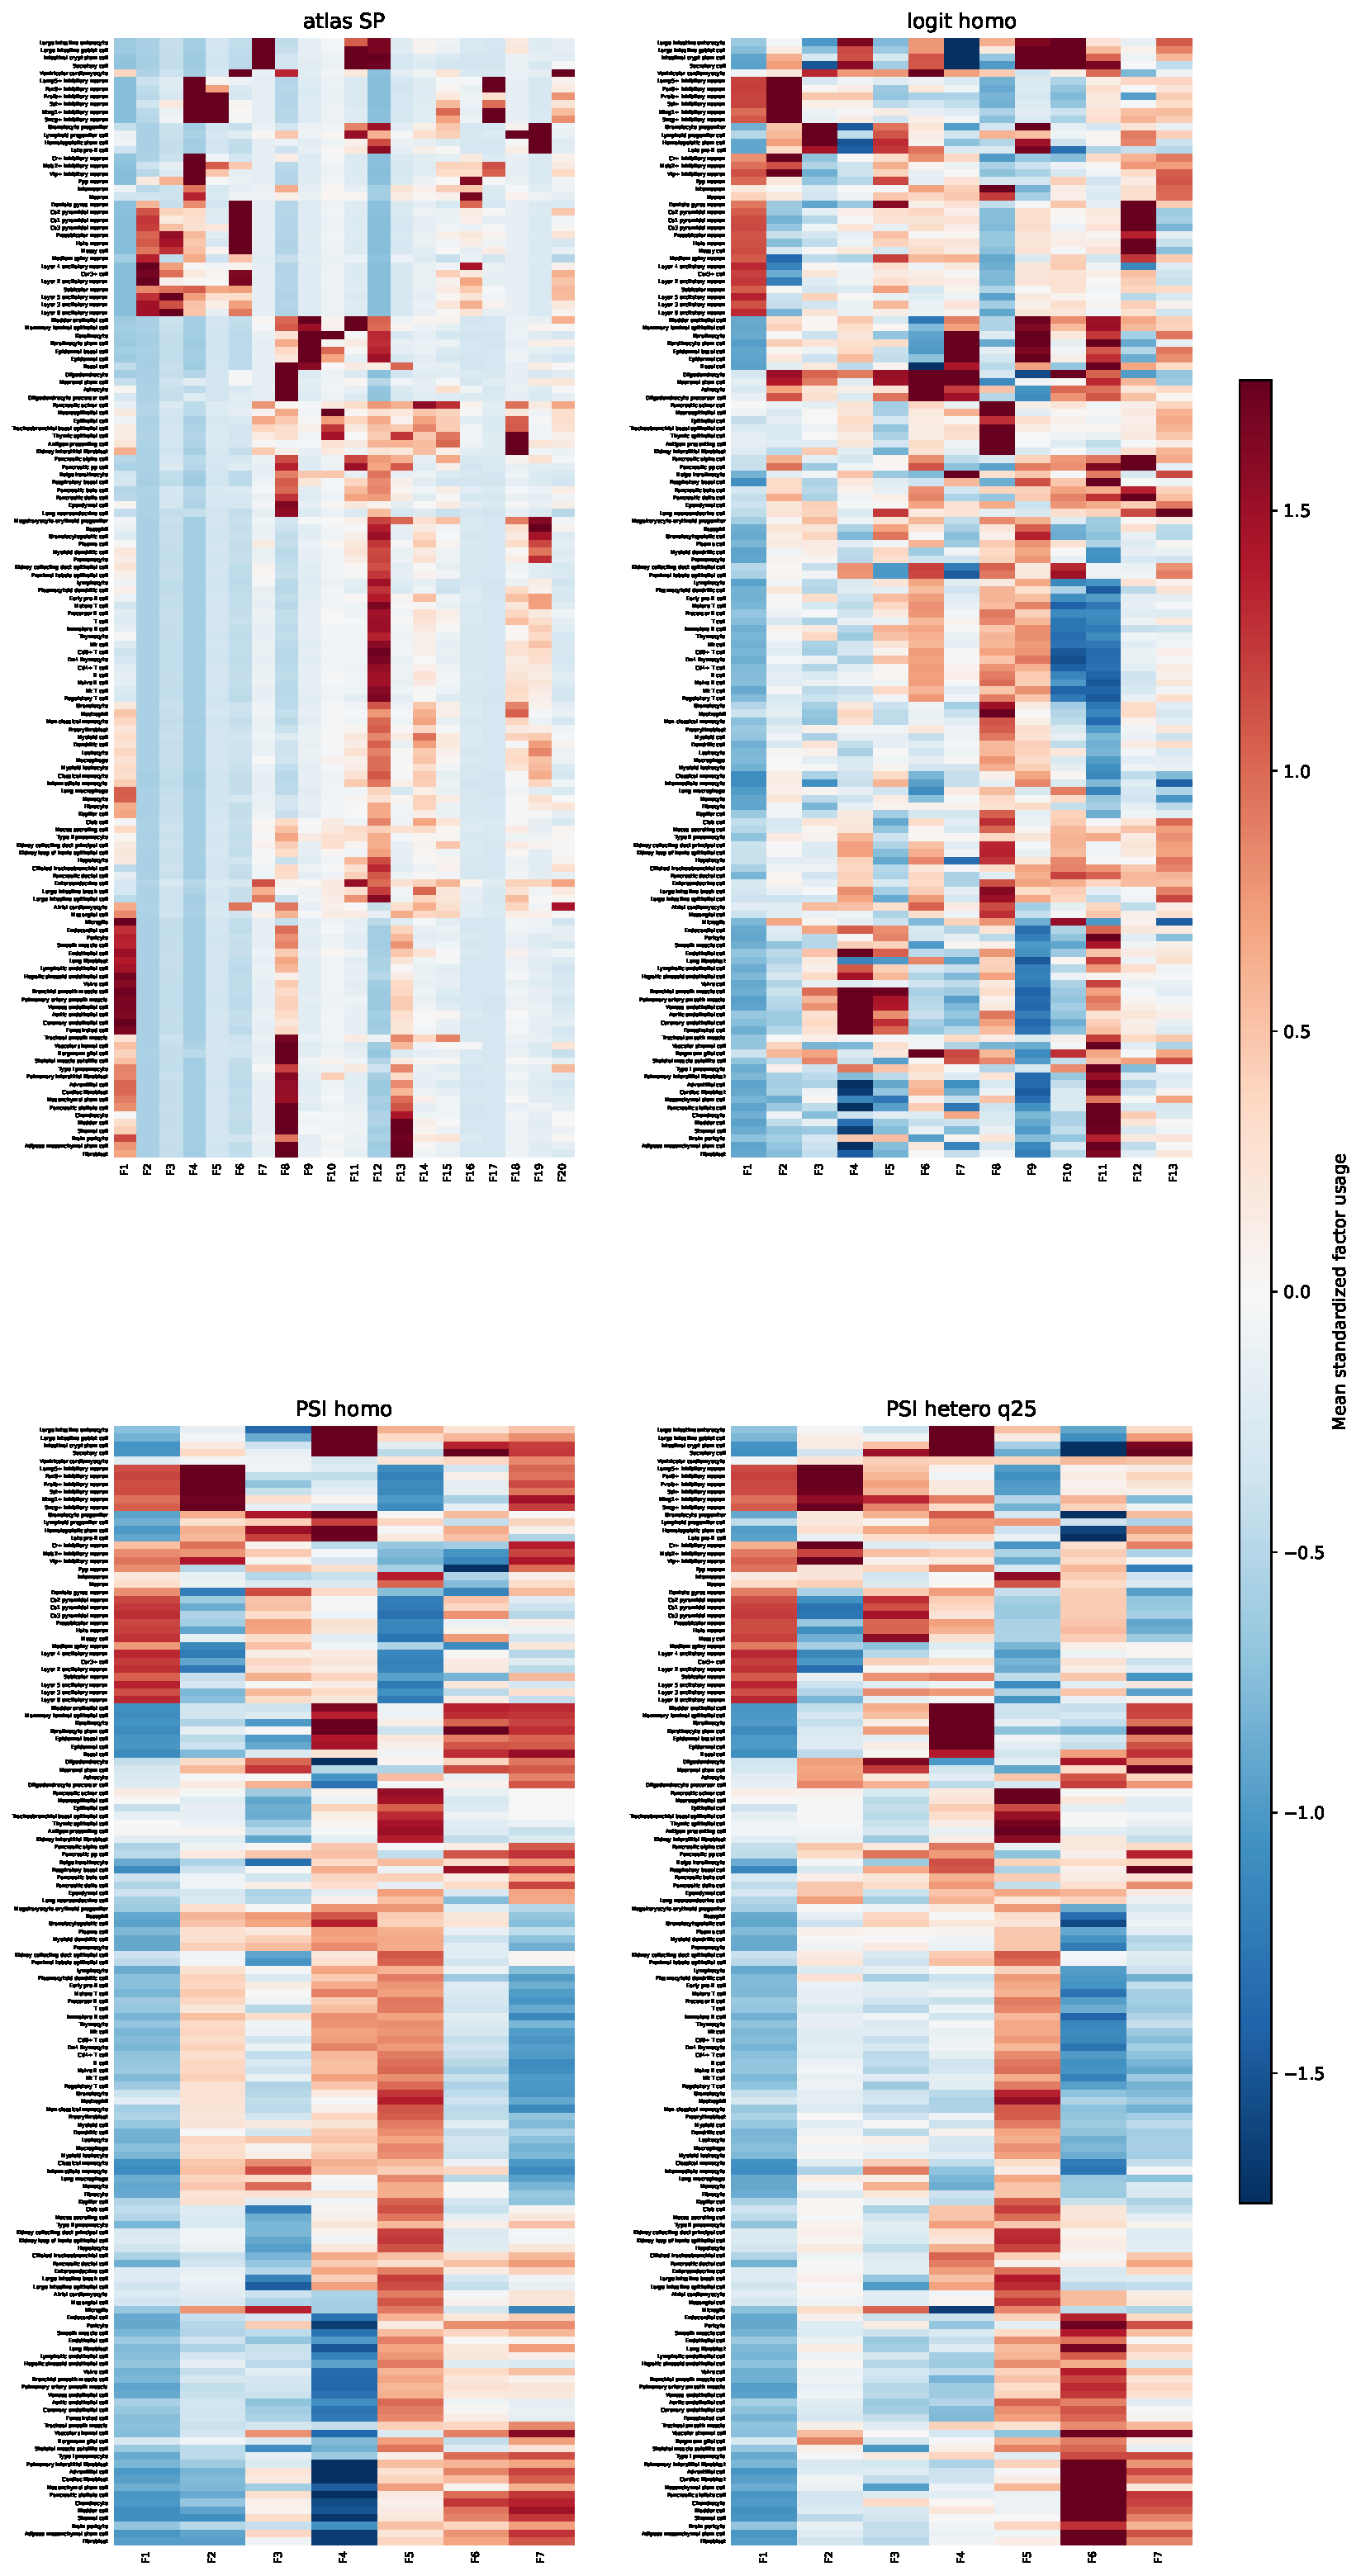
\includegraphics[width=\linewidth,height=0.9\textheight,keepaspectratio]{figures/specific_cell_type_factor_usage_heatmap.pdf}
\caption{Mean standardized factor usage by specific cell type.  This higher
resolution view contains 145 cell-type labels and is intended for zoomed
inspection in the PDF.}
\label{fig:splicing-specific-celltype-factor-usage}
\end{figure}

\subsection{Nonnegative factors from denoised proximal fits}

For interpretability, NMF and semi-NMF were fit as post-processing layers on
the PSI-scale proximal estimates.  If
\[
X_{\mathrm{prox}}=U\operatorname{diag}(d)V^\top
\]
is a fitted proximal estimate, the factorization target was generated in row
batches as
\[
\widetilde X_{i\cdot}
=
\min\{1,\max\{0, X_{\mathrm{prox},i\cdot}\}\}.
\]
Mini-batch NMF fit
\[
\widetilde X \approx WH,\qquad W\ge 0,\quad H\ge 0,
\]
with 20 nonnegative programs.  A semi-NMF variant fit
\[
\widetilde X \approx WH,\qquad W\ge 0,\quad H\in\mathbb{R}^{20\times p},
\]
so cell usages are nonnegative while junction loadings can be signed.  The
semi-NMF update alternated between projected-gradient NNLS updates for row
batches of \(W\) and a signed ridge least-squares update for \(H\).  Both
algorithms never materialized the full
\(142315\times 10000\) denoised matrix: each update generated a dense
cell-by-10000-junction block from the low-rank factors, clipped it to
\([0,1]\), and then discarded the block.  After fitting, cell usages \(W\) were
computed for all cells in row batches.

\begin{center}
\begin{tabular}{lrrrrr}
\toprule
target & method & rank & train sec. & transform sec. & eval RMSE\\
\midrule
PSI homo & NMF & 20 & 40.5 & 26.4 & 0.014\\
PSI hetero q25 & NMF & 20 & 40.7 & 27.6 & 0.009\\
PSI homo & semi-NMF & 20 & 21.3 & 5.2 & 0.0017\\
PSI hetero q25 & semi-NMF & 20 & 21.3 & 5.1 & 0.0014\\
\bottomrule
\end{tabular}
\end{center}

Both approximations therefore scale comfortably to all cells and the selected
10000 junctions.  Semi-NMF reconstructs the denoised proximal target more
closely because signed junction loadings are less restrictive.  Medium-cell-type
local purity in usage space was 0.514--0.549 for strict NMF and 0.549--0.576
for semi-NMF, compared with a random-label baseline of 0.085.  Thus the
nonnegative cell usages preserve meaningful cell-type neighborhood structure,
although less strongly than the signed proximal factors.

\begin{center}
\begin{tabular}{lrrr}
\toprule
embedding & medium purity & enrichment & silhouette\\
\midrule
NMF PSI homo & 0.514 & 6.04 & -0.195\\
NMF PSI hetero q25 & 0.549 & 6.46 & -0.211\\
Semi-NMF PSI homo & 0.549 & 6.45 & -0.213\\
Semi-NMF PSI hetero q25 & 0.576 & 6.77 & -0.203\\
\bottomrule
\end{tabular}
\end{center}

\begin{figure}[t]
\centering
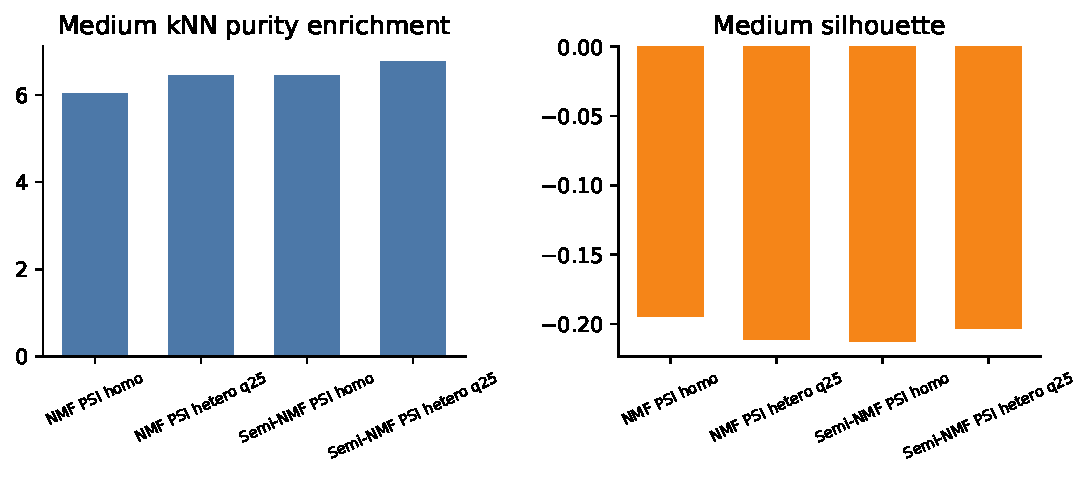
\includegraphics[width=0.78\linewidth]{figures/nmf_medium_celltype_separation_metrics.pdf}
\caption{Medium-cell-type separation metrics for nonnegative usage
coordinates.  The NMF and semi-NMF usage spaces retain substantial local cell-type
enrichment, with weaker global silhouette scores.}
\label{fig:splicing-nmf-medium-separation}
\end{figure}

\begin{figure}[p]
\centering
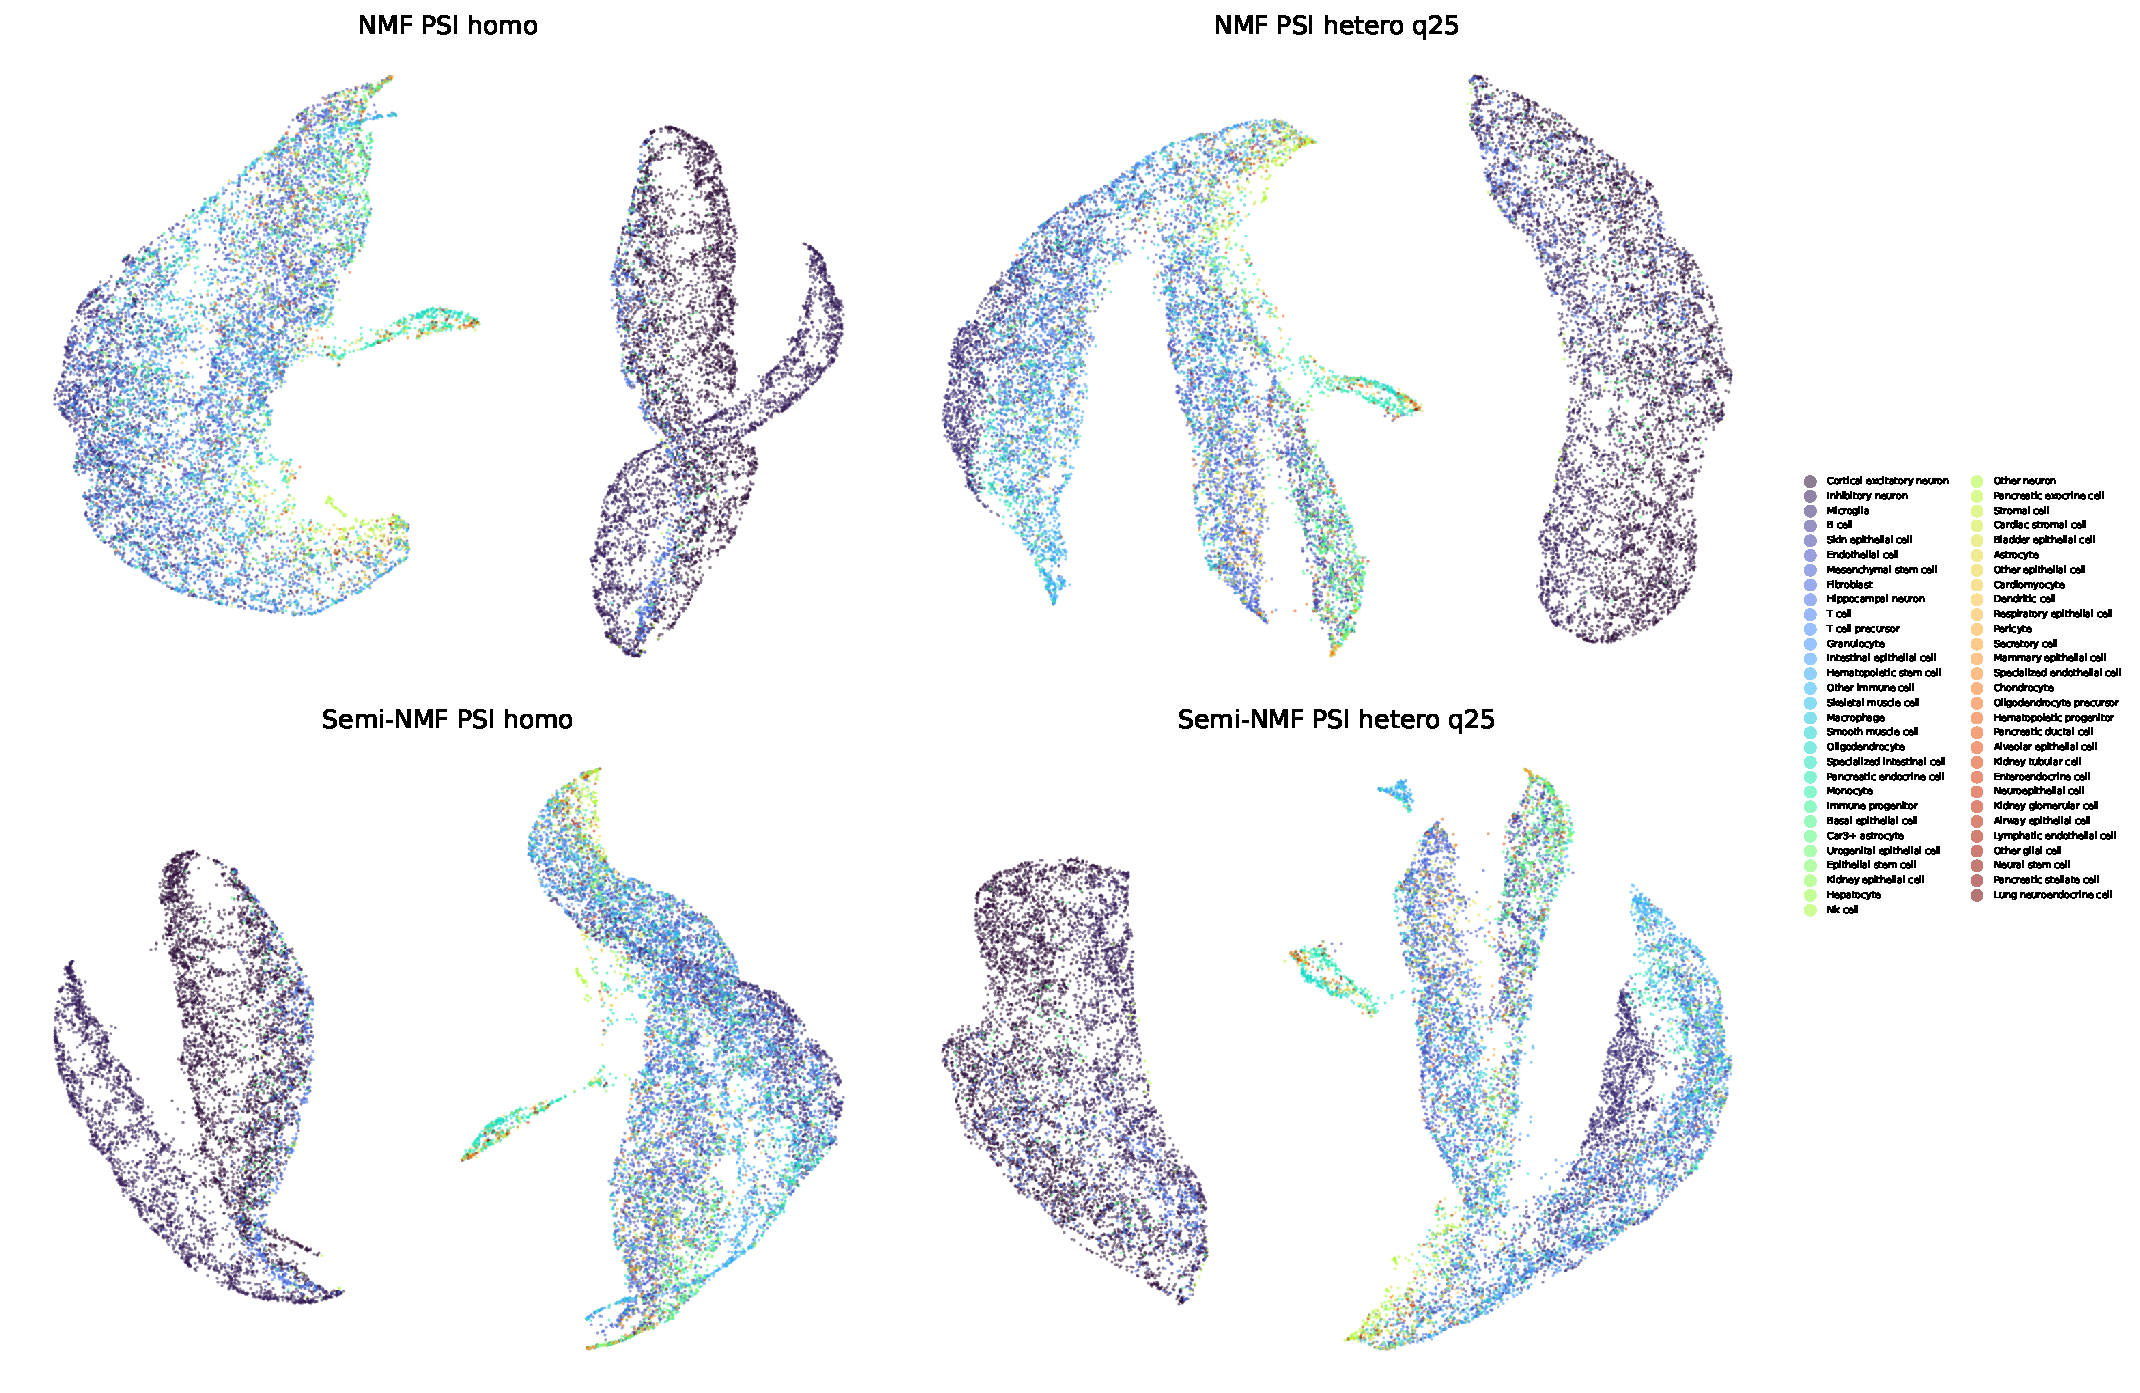
\includegraphics[width=\linewidth,height=0.9\textheight,keepaspectratio]{figures/nmf_medium_cell_type_umap.pdf}
\caption{UMAPs of rank-20 nonnegative cell usage coordinates colored by medium
cell type.  Panels compare strict NMF and semi-NMF post-processing of the
PSI-homoskedastic and PSI-heteroskedastic q25 proximal targets.}
\label{fig:splicing-nmf-medium-umap}
\end{figure}

\begin{figure}[p]
\centering
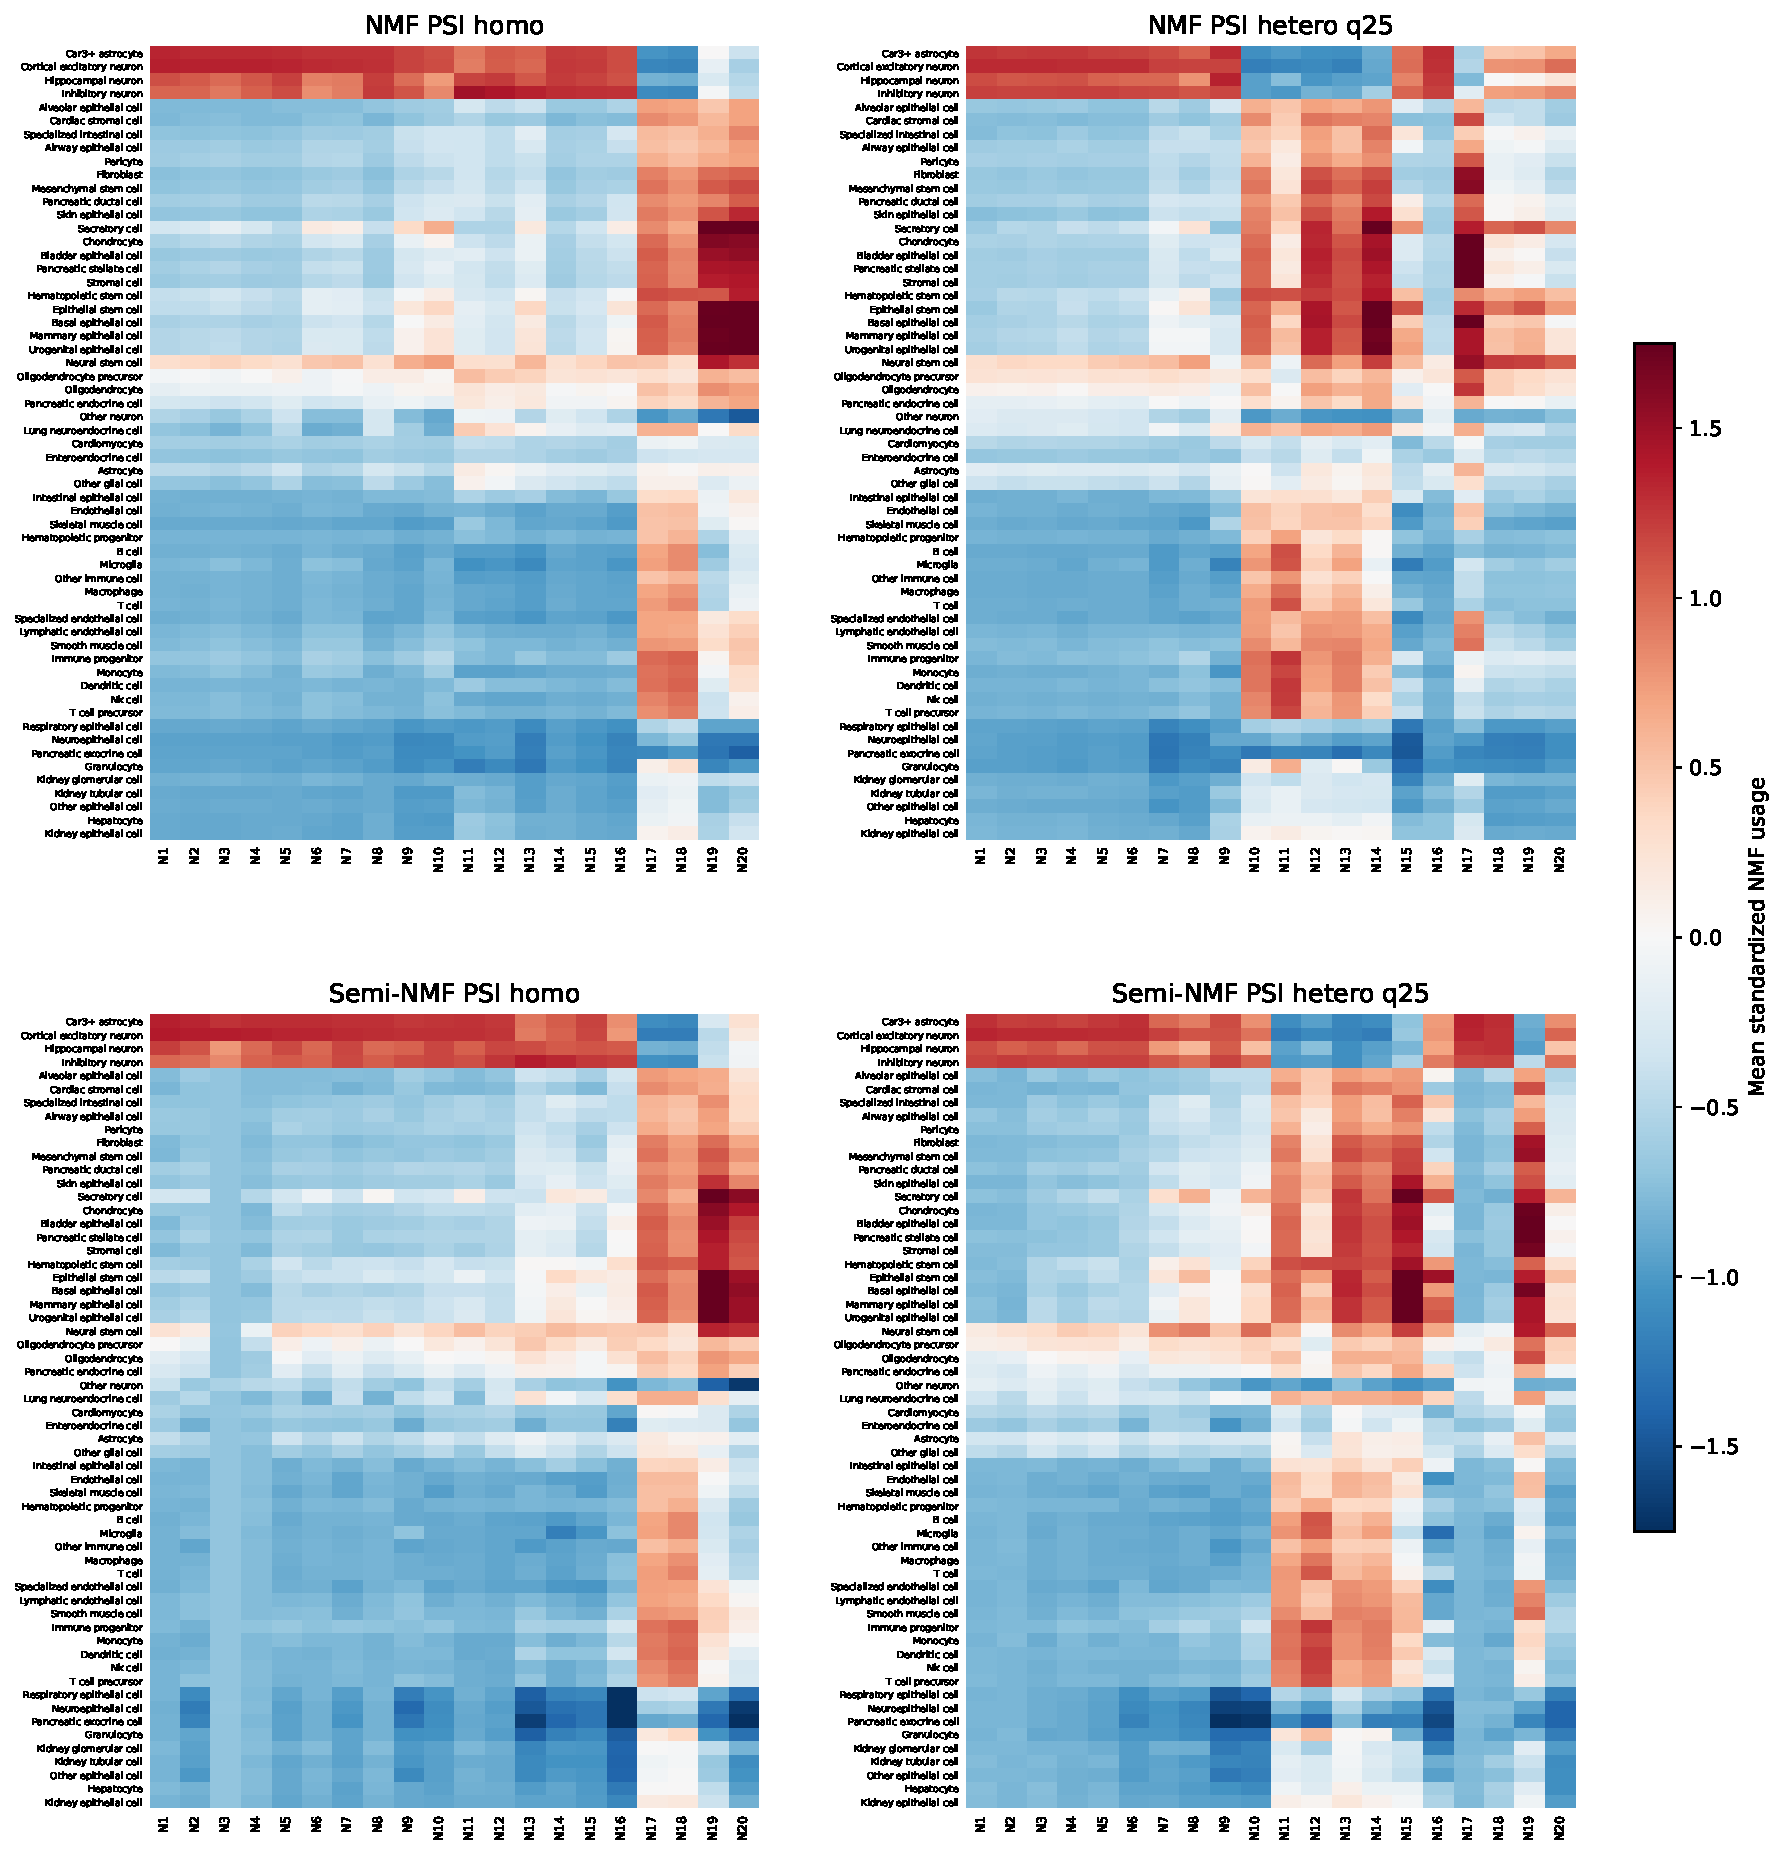
\includegraphics[width=\linewidth,height=0.9\textheight,keepaspectratio]{figures/nmf_medium_cell_type_factor_usage_heatmap.pdf}
\caption{Mean standardized rank-20 nonnegative usage by medium cell type.
Rows are medium cell types clustered by the PSI-homoskedastic NMF means.}
\label{fig:splicing-nmf-medium-factor-usage}
\end{figure}

\section{Cell-type analysis from splicing programs}

To assess whether splicing defines cell types, a multinomial logistic
classifier was trained to predict cell-type labels from the 20 fitted splicing
program coordinates in the atlas.  The final run used all available cells with
a held-out 25\% test split.  Class weights were balanced in the logistic
regression.

\begin{center}
\begin{tabular}{lrrrr}
\toprule
label & classes & accuracy & balanced accuracy & majority accuracy\\
\midrule
broad cell type & 11 & 0.767 & 0.686 & 0.255\\
medium cell type & 58 & 0.514 & 0.348 & 0.217\\
specific cell type & 132 & 0.382 & 0.263 & 0.085\\
\bottomrule
\end{tabular}
\end{center}

The 20 splicing programs are therefore strongly informative for broad cell
identity, reasonably informative for medium-resolution cell types, and still
substantially above the majority-class baseline for specific cell types.

Using all cells, the corresponding metrics were: broad cell type accuracy
0.771 and balanced accuracy 0.698; medium cell type accuracy 0.524 and balanced
accuracy 0.379; specific cell type accuracy 0.381 and balanced accuracy 0.281.

\begin{figure}[t]
\centering
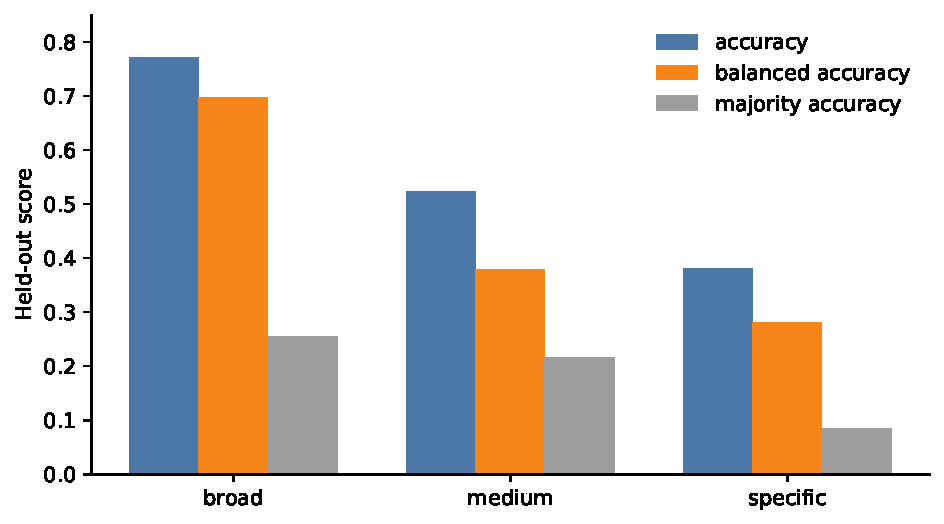
\includegraphics[width=0.7\linewidth]{figures/splicing_program_celltype_prediction.pdf}
\caption{Cell-type prediction from the 20 fitted mouse splicing programs.
Splicing programs are strongly predictive of broad cell type and remain
informative for medium and specific cell-type labels relative to the
majority-class baseline.}
\label{fig:splicing-celltype-prediction}
\end{figure}

\section{Reproducibility}

The analysis code is in \texttt{analyses/splicing\_proximal/}.  The command-line
debug run was:
\begin{verbatim}
SPLICING_MAX_CELLS=600 \
SPLICING_MAX_JUNCTIONS=200 \
SPLICING_PROX_ITER=40 \
SPLICING_LAMBDA_GRID=0.01,0.03,0.1,0.3,1 \
SPLICING_CELLTYPE_MAX_CELLS=60000 \
~/venvs/jax/bin/python analyses/splicing_proximal/run_full_analysis.py
\end{verbatim}

\end{document}
